\documentclass{acmsiggraph}
\usepackage[english]{babel}
\usepackage[T1]{fontenc}
\usepackage[latin1]{inputenc}
\usepackage{float, enumitem, footnote, multirow}
\usepackage[font=scriptsize,labelfont=bf, justification=centering, format=hang]{caption}
\usepackage{subfig}
\usepackage{amsmath, amsthm, amssymb}
\usepackage[ruled,vlined]{algorithm2e}
\usepackage{hyperref}
\usepackage{microtype}
\usepackage{lmodern}
\usepackage{listings}
\lstset{
	basicstyle=\footnotesize
}
\graphicspath{{../figures/}}

\newcommand\mycommfont[1]{\footnotesize\ttfamily{#1}}
\SetCommentSty{mycommfont}
\newcommand{\R}{\mathbb{R}}
\title{Machine Learning for Computer Vision\\ {\large [MVA 2015/2016]}\\
\vspace{10pt}
Programming Assignment 1}

\author{Maha ELBAYAD
%\\ \texttt{maha.elbayad@student.ecp.fr}}
}
\pdfauthor{Maha ELBAYAD}
\newcommand{\E}{\mathbb{E}}
\begin{document}
\maketitle

\section{Linear versus logistic regression}
Our objective is to maximize the criterion $C$ on the training set $\mathcal X = {(x_i,y_i)}_{1\leq i\leq N}$  ($x_i\in\R^d$ and $y_i\in\{0,1\}$)
\[C(w) = \sum_{i=1}^Ny_i\log\left(g\langle x_i,w\rangle\right)+(1 - y_i)\log\left(1-g\langle x_i,w\rangle\right)\]
where $g$ is the sigmoid function $g(x) = \frac{1}{1+\exp(-x)}$.\\
We can rewrite $C(w)$ as:
\[C(w) = \sum_{i=1}^N\log(1-g\langle x_i,w\rangle) + y_i \langle x_i,w\rangle\]
%\textbf{First order differential:}\\
Knowing that $g'(a) = g(a)(1-g(a))\:\forall a\in\R$
\[\nabla_wC(w) = J(w) =\sum_{i=1}^N(y_i-g\langle x_i,w\rangle)x_i \]
%\textbf{Second order differential:}\\
\[\nabla_w^2C(w)= H(w) = \sum_{i=1}^N -x_ix_i^Tg(\langle x_i,w\rangle)(1-g(\langle x_i,w\rangle)\]
if we introduce the design matrix $X = [x_1,...x_N]\in\R^{N\times d}$, the probabilities vector $G_w=[g\langle x_i,w\rangle]_i$ and $Y=[y_1,..y_N]^T$ we can deduce a matrix form for both $J$ and $H$:
\[\begin{split}
J(w) & = X^T(Y-G_w)\\
H(w) & = -X^TDX,\:D = diag(G_w\odot(1-G_w)) \\
\end{split}\]

The Newton Raphson update would be:
\[w = w_{prev} - H(w_{prev})^{-1}J(w_{prev})\]
\begin{figure}[H]
\centering
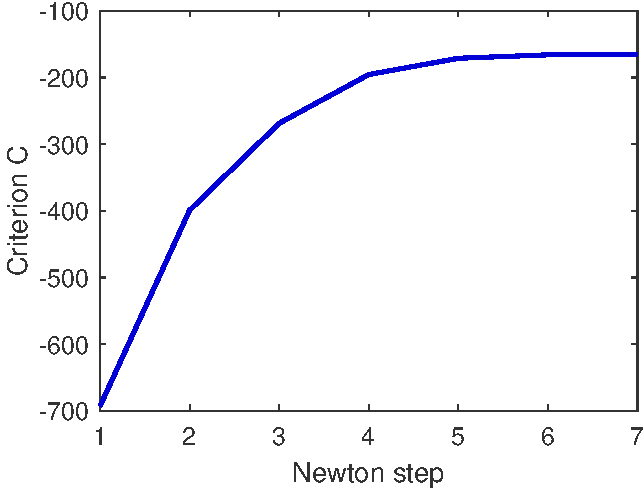
\includegraphics[height=4cm]{newton_logit}
\caption*{Newton-Raphson convergence - logistic regression}
\end{figure}
The linear regression is sensitive to the presence of outliers while the logistic regression seems more robust which leads to better accuracy
\begin{figure}[H]
\centering
\subfloat[][Logistic regression\\error rate = 6.40\%]{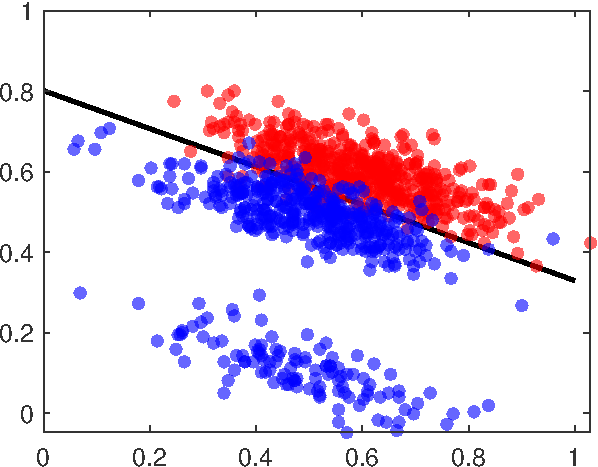
\includegraphics[height=2.8cm]{db_logit}}
\hspace{5pt}\subfloat[][Linear regression\\error rate = 11.20\%]{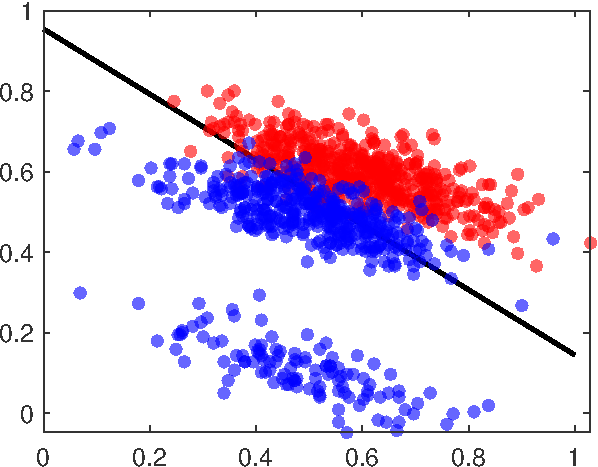
\includegraphics[height=2.8cm]{db_lr}}
%\caption{Decision boundaries}
\end{figure}
\section{Logistic Regression and Regularization}
With the additional $l_2$ regularization term:
\[\begin{split}
J(w) & = X^T(Y-G_w) - 2\lambda w\\
H(w) & = -X^TDX -2I_d \\
\end{split}\]
with a K-fold cross validation we estimate the most appropriate $\lambda$ from a set of values ranging from 1e-4 to 100:
\begin{figure}[H]
\centering
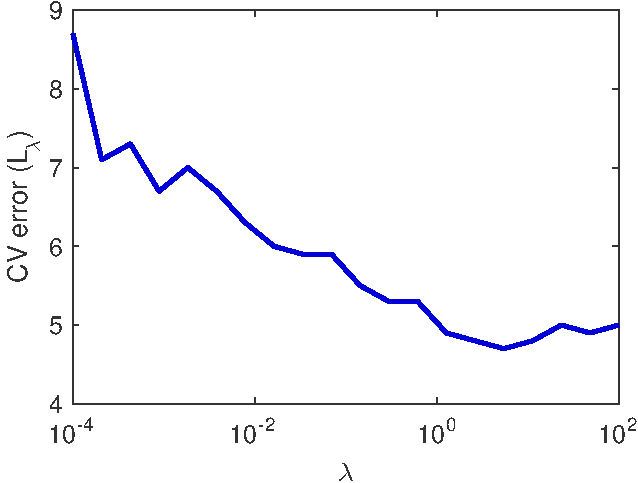
\includegraphics[height=3.6cm]{cv_error}
\caption*{K-fold average error as a function of $\lambda$\\ best performance at $\lambda^* = 5.4556$}
\end{figure}
With the logistic regression applied on a training set of size 200 with embedding dimension 241 (plus the bias term) the model overfits the data with fitted probabilities that are too close to 0/1 (an infinite criterions $C(w)$) and performs poorly on the test set.
\begin{figure}[H]
\centering
\subfloat[][Training set\\Error rate 14.5\%]{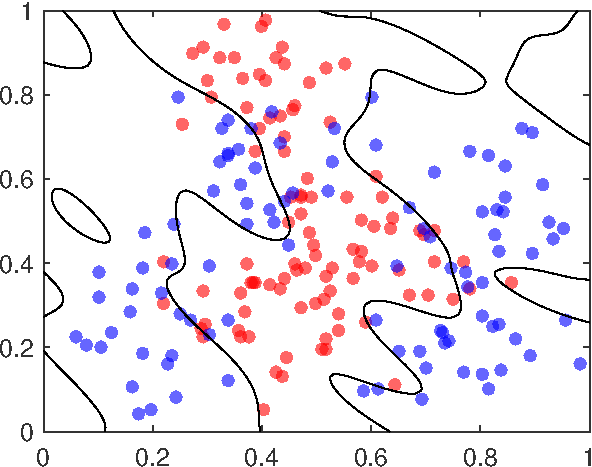
\includegraphics[height=2.8cm]{db_logit_reg}}
\hspace{5pt}\subfloat[][Test set\\Error rate 24.50\%]{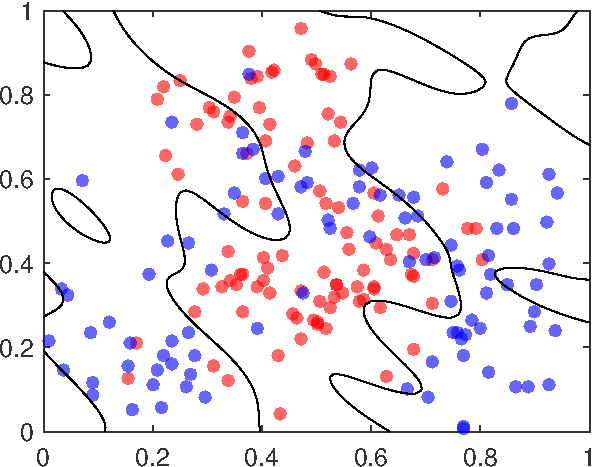
\includegraphics[height=2.8cm]{db_logit_reg_test}}
\caption*{Decision boundaries $\lambda = \lambda^*$}
\end{figure}
\end{document}